Advanced System Settings\index{advanced system settings} (Geavanceerde systeeminstellingen\index{geavanceerde systeeminstellingen}) heet niet voor niets zo. Het is een tool om settings te wijzigen die meestal niet voorkomen in Settings of Control Panel. De reden is dat het wijzigen van de settings uit Advanced System Settings je systeem negatief kan beinvloeden als je niet goed weet wat je doet. De tool is dan ook bedoeld voor IT professionals en mensen met voldoende kennis van zaken.

Om Advanced System Settings te openen:
\begin{itemize}
\item Klik op het zoek icoon en zoek op Advanced System Settings
\item Klik op het zoek icoon en zoek op System Properties
\item Gebruik de windows-toets + r en run SystemPropertiesAdvanced
\end{itemize}

\begin{minipage}[t]{\linewidth}
\raggedright
\adjustbox{valign=t}{%
	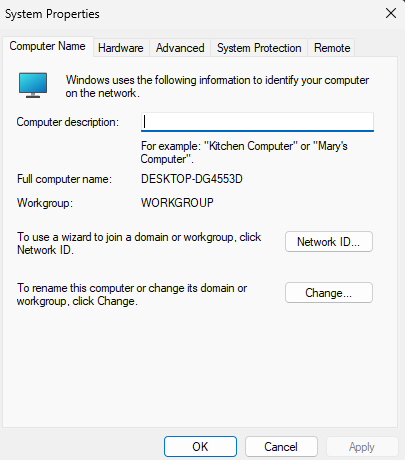
\includegraphics[width=0.99\linewidth]{advancedsystemproperties.png}%
}
\end{minipage}

